\documentclass[12pt]{article}
\usepackage[total={6in, 10in}]{geometry}

%langue
\usepackage[T1, T2A]{fontenc}
\usepackage[utf8]{inputenc}
\usepackage[english, ukrainian]{babel}

\author{студент: Недождій Олексій Сергійович \\
         викладач: Гордійко Наталія Олександрівна}
\title{Лабораторна робота № 6.1\\
    З методiв аналiзу та обробки\\
    експериментальних даних\\
       Варіант №16}
\date{}


%matlab standard
\usepackage{lmodern}
\usepackage{graphicx}
\usepackage{color}
\usepackage{listings}
\usepackage{hyperref}
\usepackage{amsmath}
\usepackage{amsfonts}
\usepackage{epstopdf}
\usepackage{matlab}

\sloppy
\epstopdfsetup{outdir=./}
\graphicspath{ {./lab6_images/} }

\begin{document}
\maketitle

\section{Завдання}
\begin{enumerate}
    \item
        Отримати з файлу mri.mat зріз черепної коробки людини та збільшити
        отримане зображення вдвічі.
    \item
        Застосувати до отриманого збільшеного зображення різні способи
        підвищення яскравості (histeq, imadjust, adapthisteq).
    \item
        Провести обробку найкращого із зображень, отриманих у п.2),
        підібравши оптимальну комбінацію цифрових фільтрів та вивести його у
        псевдокольорі. Для наочності порівняння в різні підвікна одного графічного
        вікна виводити отримані зображення та їх гістограми з пояснювальними
        надписами.
    \item
        Додати до найкращого із зображень, отриманих у п.2), різні види шуму
        (гаусівський, імпульсний, пуасонівський, мультиплікативний). Побудувати
        гістограми зашумлених зображень для всіх видів шуму та зробити висновки
        про характер розподілу яскравості пікселів залежно від виду шуму.
    \item
        провести фільтрацію зображень,
        зашумлених мультиплікативним шумом, за допомогою наступних фільтрів:
        \begin{itemize}
            \item медіанного фільтру (medfilt2);
            \item максимізуючого фільтра (ordfilt2 з відповідними параметрами);
            \item мінімізуючого фільтра (ordfilt2 з відповідними параметрами).
        \end{itemize}
\end{enumerate}

\section{Рішення}

\begin{par}
\begin{flushleft}
Завантажуєм файл
\end{flushleft}
\end{par}

\begin{matlabcode}
load mri.mat;
D=squeeze(D);
\end{matlabcode}


\begin{par}
\begin{flushleft}
Отримуєм зображення з массиву, збільшуєм в двічі
та застосовуєм різні способи збільшення  яскравості
\end{flushleft}
\end{par}

\begin{matlabcode}
img = D(:,:,16);
img = imresize(img, 2);

figure;
subplot(2,4,1);
montage(img);
title("Original");

h = histeq(img);
subplot(2,4,2);
montage(h);
title("Histeq filter");

%я гама-корекція
imad = imadjust(img);
subplot(2,4,3);
montage(imad);
title("Imadjust filter");

% автоматичне вирівнюванням гістограми
adap = adapthisteq(img);
subplot(2, 4, 4);
montage(adap);
title("Adapthisteq filter");

subplot(2, 4, 5);
imhist(img);
title("original")

subplot(2, 4, 6);
imhist(h);
title("Histeq filter");

subplot(2, 4, 7);
imhist(imad);
title("Imadjust filter");


subplot(2, 4, 8);
imhist(adap);
title("Adapthisteq filter");
\end{matlabcode}
\begin{center}
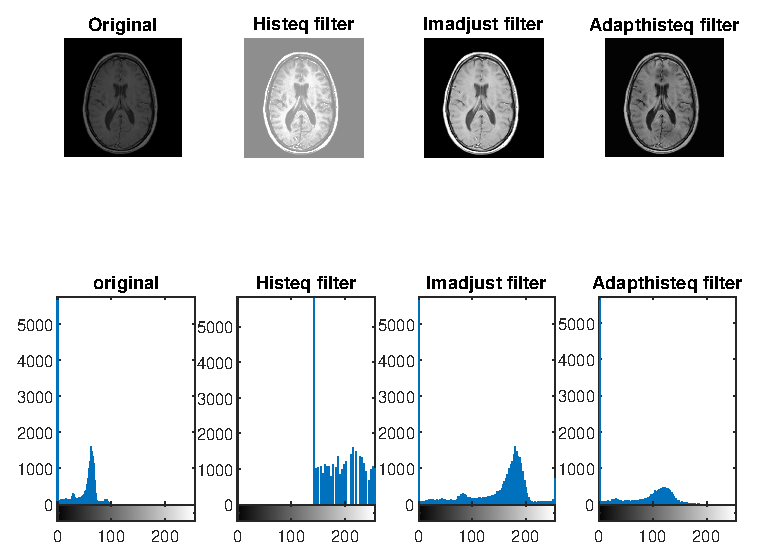
\includegraphics[width=\maxwidth{56.196688409433015em}]{figure_0}
\end{center}

\begin{par}
\begin{flushleft}
Як найкраще вибрав зображення з фільтром Adapthisteq
та застосував до нього різні типи фільтрації
\end{flushleft}
\end{par}

\begin{matlabcode}
%медіанна фільтрація
med = medfilt2(adap);
figure;
subplot(1, 2, 1);
montage(med);
title('Фільтр medfilt2')
colormap('jet');

subplot(1, 2, 2);
imhist(med);
\end{matlabcode}
\begin{center}
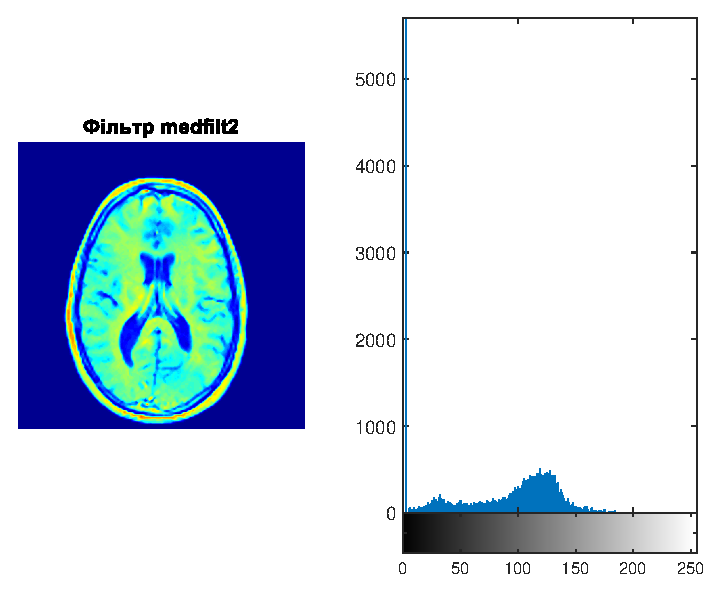
\includegraphics[width=\maxwidth{56.196688409433015em}]{figure_1}
\end{center}
\begin{matlabcode}

%адаптивна фільтрація зображення методом Вінера
win = wiener2(adap);
figure;
subplot(1, 2, 1);
montage(win);
title("Фільтр  wiener2");
colormap('jet');

subplot(1, 2, 2);
imhist(win);
\end{matlabcode}
\begin{center}
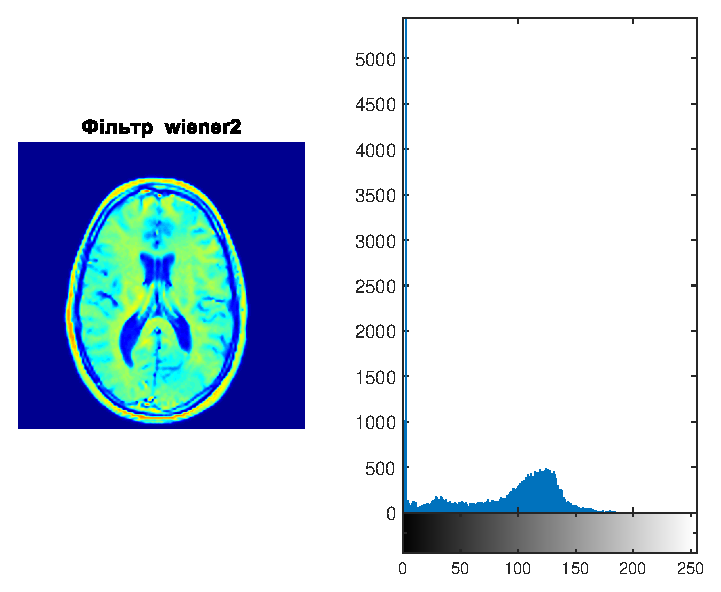
\includegraphics[width=\maxwidth{56.196688409433015em}]{figure_2}
\end{center}

\newpage
\subsection*{Добавим до зображень різні види шумів:}


\begin{par}
\begin{flushleft}
Гаусівський Шум
\end{flushleft}
\end{par}

\begin{matlabcode}
gau = imnoise(adap, "gaussian");

figure;
subplot(1, 2, 1);
montage(gau);
title("Gaussian noise");

subplot(1, 2, 2);
imhist(gau);
\end{matlabcode}
\begin{center}
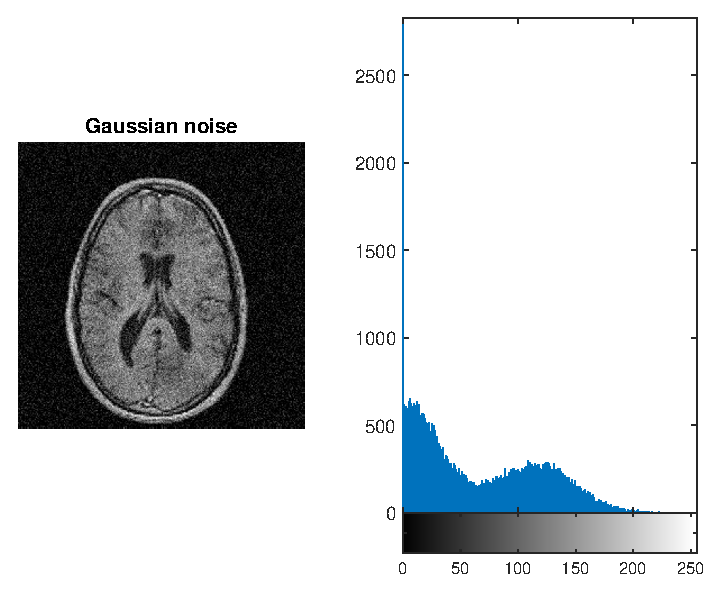
\includegraphics[width=\maxwidth{56.196688409433015em}]{figure_3}
\end{center}

\begin{par}
\begin{flushleft}
Імпульсний шум
\end{flushleft}
\end{par}

\begin{matlabcode}
imp = imnoise(adap, 'salt & pepper');

figure;
subplot(1, 2, 1);
montage(imp);
title("Impulse noise");

subplot(1, 2, 2);
imhist(imp);
\end{matlabcode}
\begin{center}
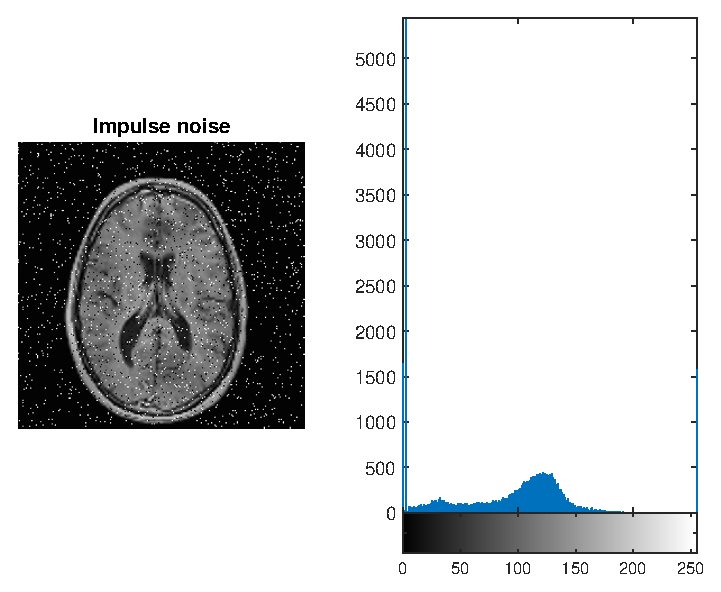
\includegraphics[width=\maxwidth{56.196688409433015em}]{figure_4}
\end{center}

\begin{par}
\begin{flushleft}
Пуасонівський шум
\end{flushleft}
\end{par}

\begin{matlabcode}
poi = imnoise(adap, 'poisson');

figure;
subplot(1, 2, 1);
montage(poi);
title("Poisson noise")

subplot(1, 2, 2);
imhist(poi);
\end{matlabcode}
\begin{center}
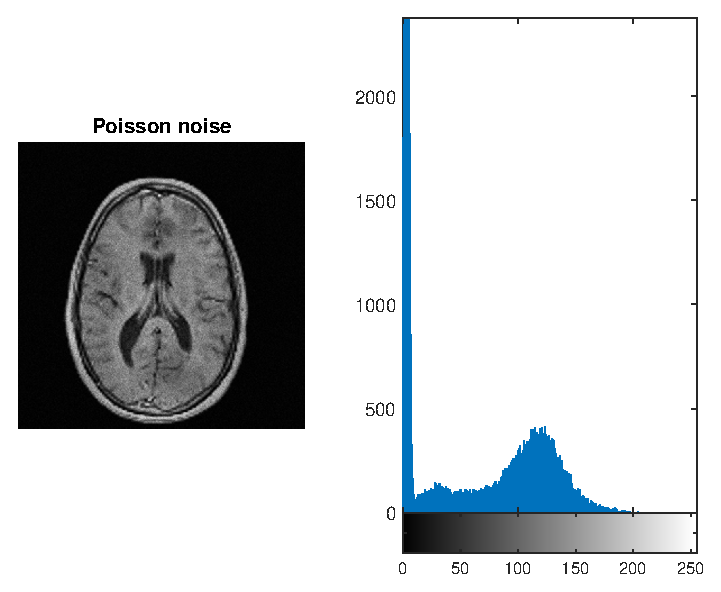
\includegraphics[width=\maxwidth{56.196688409433015em}]{figure_5}
\end{center}

\begin{par}
\begin{flushleft}
Мультиплікативний шум
\end{flushleft}
\end{par}

\begin{matlabcode}
spec = imnoise(adap, 'speckle');

figure;
subplot(1, 2, 1);
montage(spec);
title("Multiplier noise");

subplot(1, 2, 2);
imhist(spec);
\end{matlabcode}
\begin{center}
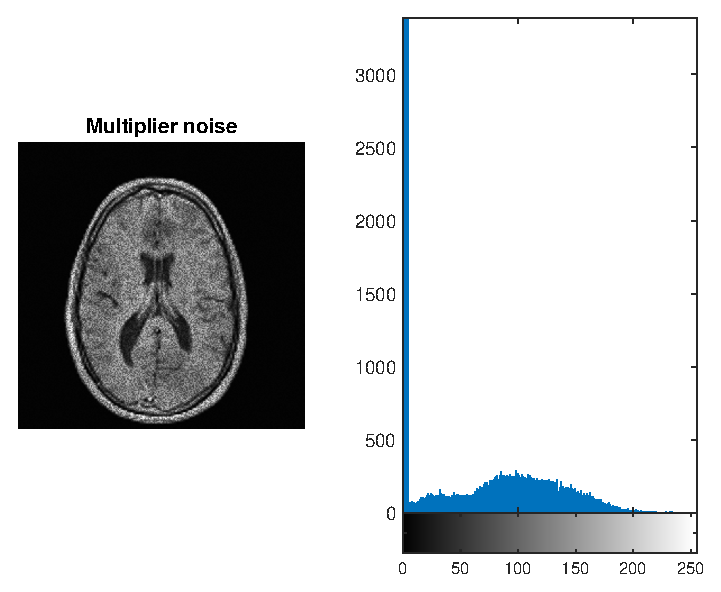
\includegraphics[width=\maxwidth{56.196688409433015em}]{figure_6}
\end{center}

\subsection*{Проводом фільтрацію зображень}
\begin{par}
\begin{flushleft}
Медіанний фільтр для зашумленого зображення
\end{flushleft}
\end{par}

\begin{matlabcode}
filter_med = medfilt2(spec);

figure;
subplot(1, 2, 1);
montage(filter_med);
title("Medfilt2")

subplot(1, 2, 2);
imhist(filter_med);
\end{matlabcode}
\begin{center}
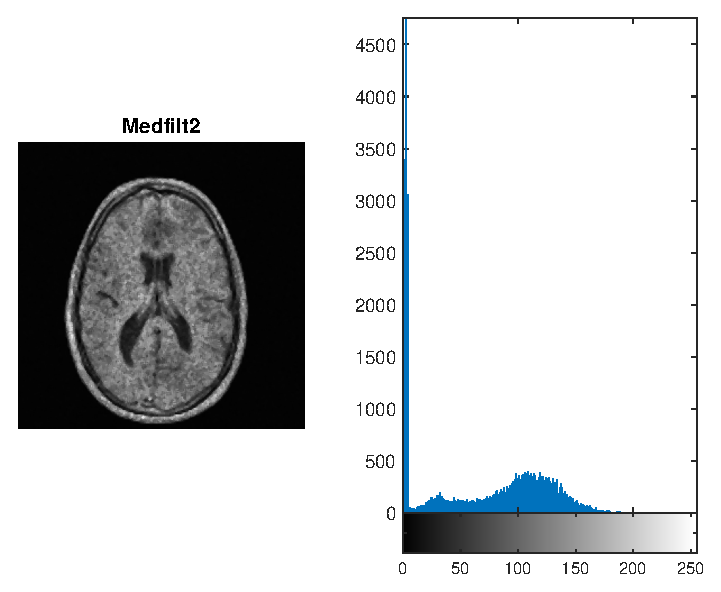
\includegraphics[width=\maxwidth{56.196688409433015em}]{figure_7}
\end{center}

\begin{par}
\begin{flushleft}
Максимізуючий фільтр для зашумленого зображення
\end{flushleft}
\end{par}

\begin{matlabcode}
filter_ord_max = ordfilt2(spec, 9, ones(3, 3));

figure;
subplot(1, 2, 1);
montage(filter_ord_max);
title("Ordfilt2 max");

subplot(1, 2, 2);
imhist(filter_ord_max);
\end{matlabcode}
\begin{center}
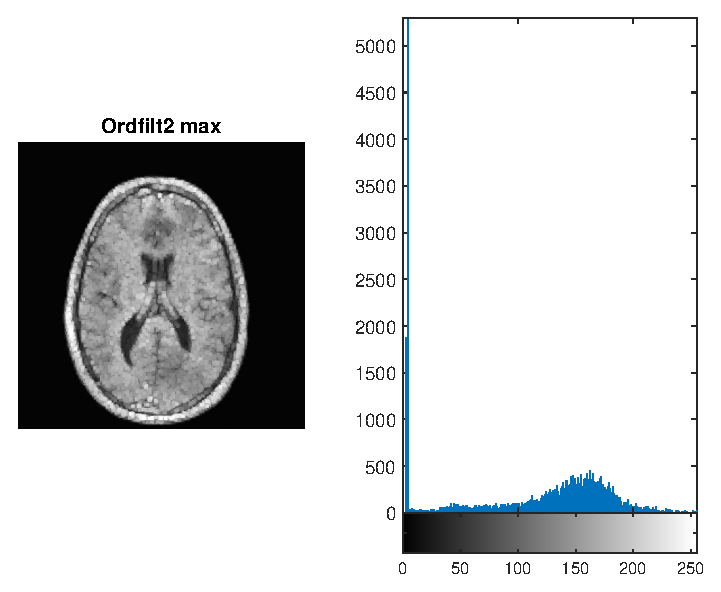
\includegraphics[width=\maxwidth{56.196688409433015em}]{figure_8}
\end{center}

\begin{par}
\begin{flushleft}
Мінімізуючий фільтр для зашумленого зображення
\end{flushleft}
\end{par}

\begin{matlabcode}
filter_ord_min = ordfilt2(spec, 1, ones(3, 3));

figure;
subplot(1, 2, 1);
montage(filter_ord_min);
title("Ordifilt2 min");

subplot(1, 2, 2);
imhist(filter_ord_min);
\end{matlabcode}
\begin{center}
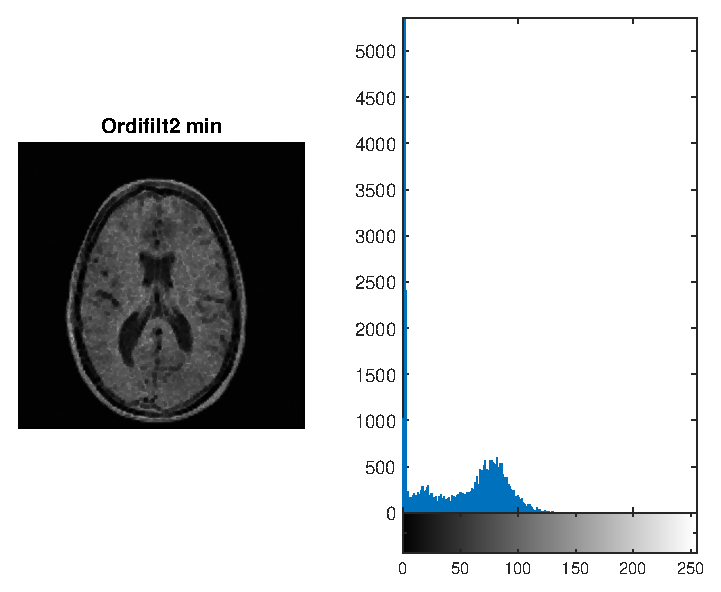
\includegraphics[width=\maxwidth{56.196688409433015em}]{figure_9}
\end{center}

\section{Висновки}
Я б обрав медіанний фільтр так як він менше змазує зображення при фільтрації.

\end{document}
